\newpage
\section{DNS}
\subsection{Introduction}
Names provide a level of abstraction from the IP address: for humans it's easier to remember. It also provides \textbf{load balancing} and easy \textbf{aliasing}.\\
The decision for DNS adding is handled by two organizations:
\begin{itemize}
	\item \textbf{IETF}: how entries are entered and read from the phone book
	\item \textbf{ICANN}: how to decide \textit{what} names should be entered in the phone book
\end{itemize}
To use naming you need two things:
\begin{itemize}
	\item \textbf{Unique} names
	\item \textbf{Resolution} of names to locator (IP address) or other services
\end{itemize}

\subsubsection{Scaling}
To allow scaling, DNS uses \textbf{delegation} and \textbf{caching}. In particular for delegation, DNS adopts three intertwined \textbf{hierarchies}:
\begin{itemize}
	\item \textbf{Name space}: hierarchy of names
	\item \textbf{Management}: hierarchy of authorities over names. Who owns which name part.
	\item \textbf{Infrastructure}: hierarchy of DNS server. Where is the mapping stored.
\end{itemize}

\subsection{Namespace}
DNS namespace is implemented as a tree structure: each node has a \textbf{label} which identifies it relatively to its parent node. Each node is \textbf{root} of a sub-tree (if it's not a leaf). In particular direct children of the root are called \textbf{Top Level Domains}. Each subtree represents a \textbf{domain} and each domain can be divided in \textbf{sub-domains}.
\begin{center}
	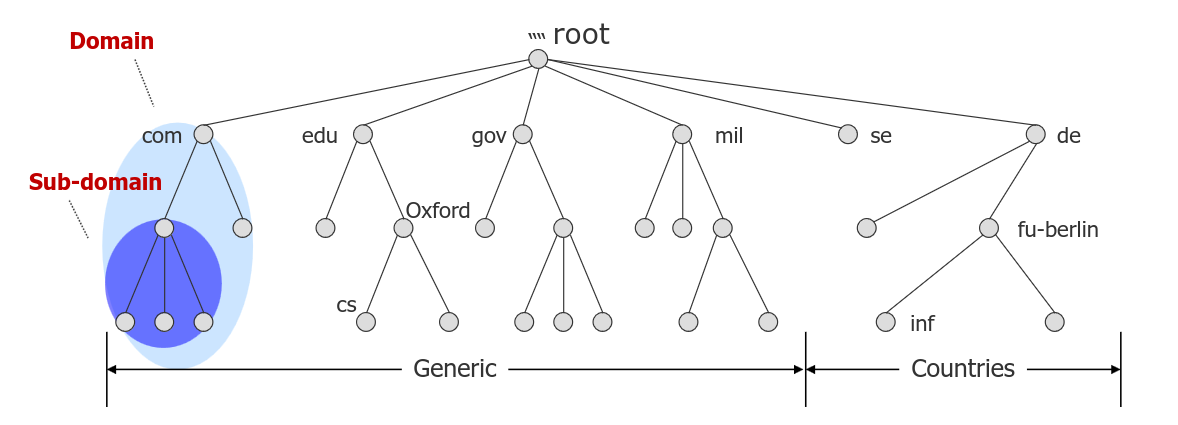
\includegraphics[scale=0.3]{dns_hier.png}
\end{center}
There is a limited number of TLDs: originally it was $7$ plus one for each country. Now there are many more, even in non Latin alphabets.
\subsubsection{Leafs}
The name of a domain consists of a sequence of labels beginning with the root of the domain and going up to the root of the whole tree. Each label is separated by ".".\\
In the leaf nodes the IP addresses are associated with the names.\\
Furthermore, there could be \textbf{Domain Name Aliases}: pointers of one domain to another (Canonical Domain Name).

\subsubsection{DNS Database}
There are a few rules for the database:
\begin{itemize}
	\item The \textbf{depth} of the tree is limited to $127$
	\item Each label can have up to $63$ characters
	\item The whole domain name has a maximum of $255$ characters (even if the average is $10$)
	\item A label of length $0$ is reserved for the root
\end{itemize}
The full address to a host is the \textbf{Fully Qualified Domain Name}, which includes the leaf, each node and the root. The \textbf{Relative Domain Name} instead, is an incomplete domain name.

\subsection{Management}
The management of domain names also follows a hierarchy structure: \textbf{ICANN} manages the root domain and delegates someone (\textbf{DENIC} for Germany) to handle the \textit{de} domain. They then delegate FUB to handle the \textit{fu} domain. And so on.\\
This solution ensures that the names are unique.

\subsection{Name servers and zones}
\subsubsection{Domains}
Domains are administrative concepts managed by single organizations. The name of the domain corresponds to the name of the root node. They can delegate the responsibility for subdomains to other organizations but maintains the pointer to them to be able to forward requests.
\subsubsection{Name servers and zones}
On the other hand, name servers and zones are technical concepts. The name server is a process that maintains a database for a domain space. The part of the name space known to the server is called a \textbf{zone} and it's stored in a \textit{zone file}. The name server may have multiple zones and has authority over them.
\paragraph{Primary Master} It's a name server that must exist. Reads the data from a local file and has a database describing subdomains and computer in a selected zone.
\paragraph{Secondary Master} It's optional and is a replication of the master for reliability reasons. It receives the data from another server which is authoritative.

\subsection{Resolution}
There are two types of Name Resolution:
\begin{itemize}
	\item \textbf{Recursive}: the name server replies either with the answer or with an error and it's responsible to contact the other nodes
	\item \textbf{Iterative}: a name server replies with the address of another one, it's the host duty to contact additional name servers for the answer
\end{itemize} 

\begin{question}[Why do root servers not support recursive solution?]
	Using the recursive option implies that every intermediate needs to wait for all the others, depleting its resources.
\end{question}

\begin{question}[How does this all contribute to scalability?]
	We do not have \textbf{strong consistency} and 
\end{question}

\subsubsection{Reverse lookup}
While mapping a name to a \textit{global} IP address is simple, doing the other way round it's really difficult because we need to do a complete search of the tree. \\
Because of this, there is a special area in the database called \textbf{in-addr.arpa} that contains $256$ sub domains, each one having $256$ and so on.
\begin{center}
	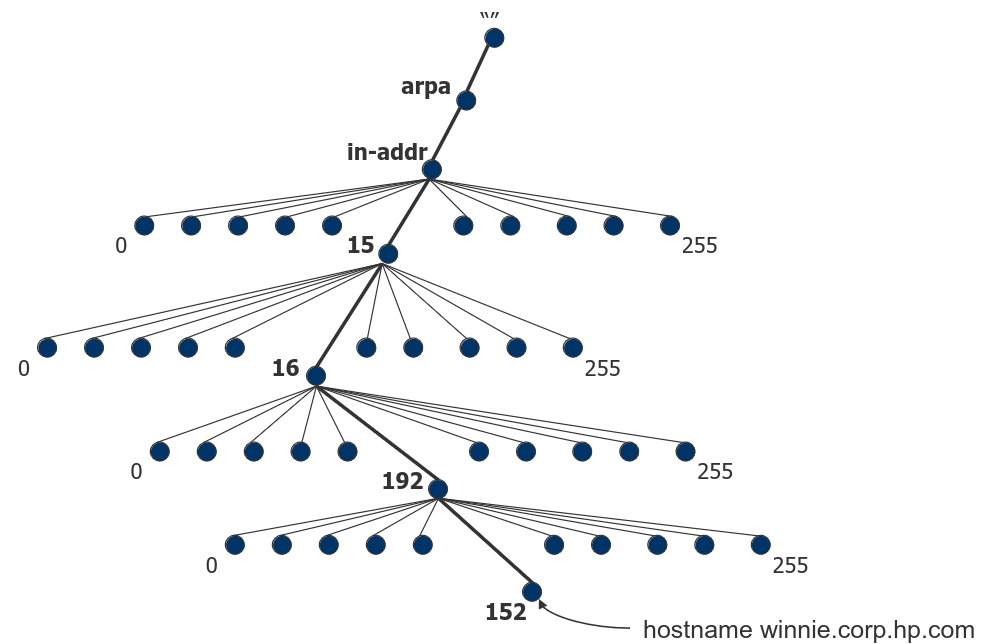
\includegraphics[scale=0.3]{reverselookup.png}
\end{center}
\begin{note}
	This is useful against \textbf{spoofing}: as an example if you get an email and you want to check if the sender is who claims to be, you can do a reverse lookup on the IP of the email server.
\end{note}

\begin{question}[Why does reverse lookup not always work?]
	Because the entries are not always present in the database.
\end{question}

\subsection{Database entries}
A \textbf{resource record} is the entry in the database to get the address or other information of a name. It's composed of a tuple:
\begin{lstlisting}[language=Python]
	(name, TTL, class, type, value)
\end{lstlisting}
\paragraph{TTL} It's the Time To Live: after a certain amounts of seconds the record will be deleted from the cache and updated. With a shorter TTL you have a very updated cache while longer TTL means outdated caches but less requests for the server.
\paragraph{Type} Indicates the type of data to be returned. \textbf{A} is the actual IPv4 address corresponding to the name (\textbf{AAAA} for IPv6). 
\paragraph{Class} Nowadays it's only \textbf{IN} but there were in the past other options for different networks with independent DNS zones.

\begin{observation}[Load balancing]
	DNS is very useful for load balancing: depending on the region when you ask for a DNS entry the answer will be the closest one. It can also be used for \textbf{evil purposes} (censorship, marketing).
\end{observation}

\subsubsection{Name Server}
For each name server of a zone a \textbf{Name Server} record is created in the cache. E.g. when you want to visit \textit{arnold.movie.edu} you may have in cache a NS entry for \textit{movie.edu}.

\subsubsection{CNAME}
A \textbf{CN} record is an optional entry in the database that illustrates aliases on its canonical names. 

\subsubsection{Pointer}
The \textbf{PTR} record provides information for the mapping of an address to names. If you do not have any entry for an IP address you then have to do a reverse lookup. Addresses should refer only to one name.

\subsubsection{Mail Exchanger}
The \textbf{MX} record serves for the controlling of the email routing. It specifies an email server responsible for a domain name with the option to indicate a preference if multiple servers are present (the smallest value is preferred).

\subsection{Protocol}
The resolver software triggers the resolution process and tries first for the cache. Then it sends the request to the local DNS server which is either static (resolv.conf) or dynamic (DHCP). \\
The protocol consists of a single packet used for inquiries and responses:
\begin{center}
	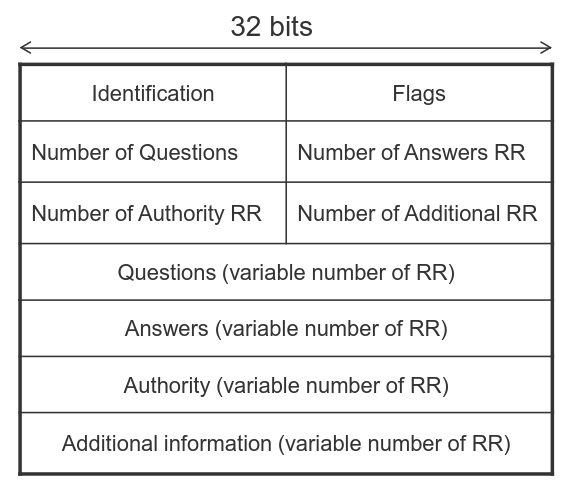
\includegraphics[scale=0.3]{dns.png}
\end{center}
\paragraph{Identification} $16bits$ for the mapping of an inquiry to a response.
\paragraph{Flags} $16bits$ of various flags that indicate if the packet is a request or a response, if it's \textbf{authoritative} or not, if it's \textit{iterative} or \textit{recursive}.
\paragraph{Numbers} These fields indicate the contained number of inquiries responses data records.
\paragraph{Questions} Contains the names to be resolved.
\paragraph{Answers} Resource records to the previous inquiry.
\paragraph{Authority} Contains the ID of the passed responsible NS.
\paragraph{Additional information} If the name searched is only an alias, the belonging resource record for the correct name is placed here.

The packet is sent through UDP on port $53$ and the \textbf{reliability} is only implemented via repeating the requests. Also it is not protected.

\subsection{Scalability}
The scalability is achieved mainly with local caching of recent results. The cache can be in the network and also in the local client.\\
One of the main problem is how long should you keep the entries? You need to achieve both \textbf{consistency} and not doing too many requests. You also need to detect and flush the \textbf{stale entries}. You have to avoid \textbf{cache poisoning}: when a malicious person changes the value in the cache to redirect you to an evil software.
\subsection{Extension}
\subsubsection{Dynamic DNS}
The problem comes up when, as an example, you restart the router and your public IP address is changed (or maybe the ISP changes it every 24 hours). The DDNS allows you to tell the changed IP address.
\subsubsection{Characters}
The original DNS supports only ASCII, so there is an extension for UTF characters.
\subsubsection{DNSSEC}
The \textbf{security} is important because DNS is the most crucial indirection to access the data. Controlling DNS response implies controlling the discovery of the communication endpoints. It may be use in an evil way for political and economical reasons.